%\documentclass{tise_style}
%\usepackage{natbib}
%Having trouble getting tise_style to compile correctly in RStudio, will re-run it with this before submission

%-----------------------------------------------------------------------------------------------------
%Substitute this all with tise_style
\documentclass[12pt]{article}\usepackage[]{graphicx}\usepackage[]{color}
%% maxwidth is the original width if it is less than linewidth
%% otherwise use linewidth (to make sure the graphics do not exceed the margin)
\makeatletter
\def\maxwidth{ %
  \ifdim\Gin@nat@width>\linewidth
    \linewidth
  \else
    \Gin@nat@width
  \fi
}
\makeatother

\definecolor{fgcolor}{rgb}{0.345, 0.345, 0.345}
\newcommand{\hlnum}[1]{\textcolor[rgb]{0.686,0.059,0.569}{#1}}%
\newcommand{\hlstr}[1]{\textcolor[rgb]{0.192,0.494,0.8}{#1}}%
\newcommand{\hlcom}[1]{\textcolor[rgb]{0.678,0.584,0.686}{\textit{#1}}}%
\newcommand{\hlopt}[1]{\textcolor[rgb]{0,0,0}{#1}}%
\newcommand{\hlstd}[1]{\textcolor[rgb]{0.345,0.345,0.345}{#1}}%
\newcommand{\hlkwa}[1]{\textcolor[rgb]{0.161,0.373,0.58}{\textbf{#1}}}%
\newcommand{\hlkwb}[1]{\textcolor[rgb]{0.69,0.353,0.396}{#1}}%
\newcommand{\hlkwc}[1]{\textcolor[rgb]{0.333,0.667,0.333}{#1}}%
\newcommand{\hlkwd}[1]{\textcolor[rgb]{0.737,0.353,0.396}{\textbf{#1}}}%
\let\hlipl\hlkwb

\usepackage{framed}
\makeatletter
\newenvironment{kframe}{%
 \def\at@end@of@kframe{}%
 \ifinner\ifhmode%
  \def\at@end@of@kframe{\end{minipage}}%
  \begin{minipage}{\columnwidth}%
 \fi\fi%
 \def\FrameCommand##1{\hskip\@totalleftmargin \hskip-\fboxsep
 \colorbox{shadecolor}{##1}\hskip-\fboxsep
     % There is no \\@totalrightmargin, so:
     \hskip-\linewidth \hskip-\@totalleftmargin \hskip\columnwidth}%
 \MakeFramed {\advance\hsize-\width
   \@totalleftmargin\z@ \linewidth\hsize
   \@setminipage}}%
 {\par\unskip\endMakeFramed%
 \at@end@of@kframe}
\makeatother

\definecolor{shadecolor}{rgb}{.97, .97, .97}
\definecolor{messagecolor}{rgb}{0, 0, 0}
\definecolor{warningcolor}{rgb}{1, 0, 1}
\definecolor{errorcolor}{rgb}{1, 0, 0}
\newenvironment{knitrout}{}{} % an empty environment to be redefined in TeX

\usepackage{alltt}
\usepackage{natbib}  % used for citations
\usepackage[parfill]{parskip} %used for formatting style of text
\usepackage{url}
\usepackage{graphicx}
\usepackage{setspace}
\usepackage{fancyvrb}
% Sets margins to 1 in
%\addtolength{\oddsidemargin}{-.5in}%
%\addtolength{\evensidemargin}{-.5in}%
%\addtolength{\textwidth}{1in}%
%\addtolength{\textheight}{1.3in}%
%\addtolength{\topmargin}{-.8in}%
%-----------------------------------------------------------------------------------------------------



\title{DataCamp: An Interactive Teaching Tool}

\author{Tessa Mcdonnel, Shannon Pileggi \\Statistics Department \\ California Polytechnic State University, San Luis Obispo}

\IfFileExists{upquote.sty}{\usepackage{upquote}}{}
\begin{document}


\maketitle

\section{Introduction}

\doublespacing

It is no surprise that technology plays a vital role in the field of statistics. As the technological revolution continues to
unfold, the use of statistical software has become increasingly emphasized in education \citep{AmericanStatisticalAssociation2016}. By integrating the
capabilities of technology in statistics courses, students can explore fundamental concepts by analyzing and
interpreting real data sets \citep{Chance2007, Hardin2015, Horton2014}, giving them an authentic view of how statistics is 
practiced outside of the
classroom \citep{Wang2017}.

The goal of any statistics course is to help students develop the ability to think statistically
\citep{AmericanStatisticalAssociation2016}; introducing technology into the curriculum can greatly strengthen this ability by illustrating concepts such as
variability, randomness and hypothesis testing. Although numerous statistical technologies exist, R and R Studio
provide extensive computational abilities (free of charge) and are commonly used in statistics courses. R
allows students to explore real-world data sets which can not only enhance their understanding of concepts, but can also spark
an interest in the domain of statistics \citep{Wang2017}.


\subsection{Interactive tools to learn R}
With the increased use of R in classrooms, an effective tool to familiarize students with statistical software is needed
\citep{Baumer2014}. While R software provides users with extraordinary statistical capabilities, there is certainly a steep learning curve. To facilitate
this transition to R programming, popular interactive teaching technologies have been created including \textit{swirl} \citep{Kross} and Try R \citep{TryR}. 
Interactive tools allow students to actively work through coding problems while receiving immediate feedback.

\subsubsection{\textit{swirl}}
\textit{swirl} \citep{Kross} is an
open source R package where students can learn R programming directly in the R console. This interactive learning tool
contains several pre-existing lessons but educators can also create their own
lesson content to fit specific curriculum \citep{Carchedi2014}.
While \textit{swirl} can be linked to Massive Open Online Courses (MOOCs) like Coursera, integration of learning management 
systems (LMS) is not available currently. 

\subsubsection{Try R}
Try R \citep{TryR} is another interactive R programming course but unlike \textit{swirl}, Try R is web-based. 
The R console can be intimidating to
new statistics students so an advantage of a web-based teaching tool is
the clean and easy to use interface. User-friendliness is an important quality given that students often struggle more with the
software used than the statistical concepts themselves \citep{Hare2017}. When students only need their web browser to participate,
all installation complications are avoided and valuable class time can be focused on the lesson.
However, Try R is not open source so public content authoring
is not available; educators are limited to the existing lessons available on the Try R website. 

\section{Introduction to DataCamp}

The purpose of this article is to introduce a new interactive teaching technology, DataCamp.
In addition to R, DataCamp offers courses in other programming languages including Python and SQL for data science.
\subsection{DataCamp course features}

DataCamp provides the same reproducible capabilities as \textit{swirl} but is a web-based application. Educators can
create their own courses that coincide with specific lessons and students can access the course without installing any software.
Courses are available through the DataCamp website so students can access the lesson through their web-browser on a laptop,
tablet or mobile device, making the courses accessible to anyone with an internet connection. These programming courses can be used in the 
classroom in a number of ways: as traditional homework assignments, as an activity during lab periods, as pre-class assignments
for a flipped classroom, and even as a test or assessment tool.


\subsubsection{Introduction to DataCamp - don't know what that note says?}
DataCamp website offers free "community" courses as well as more specialized \textit{Premium} classes that require a fee. 
However, when used for academic purposes the \textit{Premium} DataCamp content is free for up to six months.
College educators can create a classroom group on the DataCamp website, add students to the group, 
assign any of the existing courses and even assign a course that they have developed themselves. 
The collection of community courses available on DataCamp include a wide range of topics from \textit{Introduction to R} to
\textit{Quantitative Risk Management in R} so novice through advanced programming students benefit.

\subsubsection{Modularity}
DataCamp courses are broken up into chapters and each chapter is composed of modular exercises. Modularity is a critical component in designing a
learning tool because it allows independent pieces to be added, modified or removed from the entire functionality
\citep{Hare2017}. DataCamp course exercises can be added, modified, or deleted as new topics arise and instructors can tailor
these exercises to meet the needs of a particular class. The only disadvantage of the modularity feature is that the sessions
are not cumulative; every exercise begins with a clear work space so an object defined in a previous exercise needs to be
defined again.

\subsubsection{Gamification}
Each chapter exercise is given a specified number of redeemable points which the students can see when they begin
the exercise, introducing a gamification feature to the learning experience. When in a classroom group, students can view their
progress (points and chapters completed) as well as the progress of their peers. Students will often perform better
in order to be on par with the rest of the class. Furthermore, when students can see the number of available points
for an exercise it can motivate them to meet their personal achievement goals. \citep{Chang2016}. If the student completes an exercise without
any assistance, they will receive the full points. If the student is having trouble with a problem, they can view the exercise `hint' option and 30 percent
of the available points are deducted; all points are deducted if they ask for the solution. 

\subsubsection{Integration with Learning Management Systems}
One feature that sets DataCamp apart from competing technologies is the ability to track student progress. Educators
can set deadlines for assignments and view which sections the
students had trouble with in a detailed report. DataCamp courses can also be linked to the school's learning management system (LMS), such as Moodle or Blackboard, so student scores are automatically updated to the
current grade-book, allowing for a smooth integration of student work.


\subsection{Pre-existing R courses}
In order to utilize 
DataCamp's \textit{classroom} benefits, first create an academic group on the website \url{https://www.datacamp.com/groups/education}.
After your university information has been verified and the classroom account has been approved, access is facilitated 
by adding students to the DataCamp group by supplying university email addresses on the \textit{Members} tab, or by creating an integration to your LMS.
\section{Creating a DataCamp Course}
\subsection{Getting Started}
To build a course on DataCamp you will first need to create a DataCamp account by visiting \url{www.datacamp.com/teach} as well as
a GitHub account (\url{https://github.com}). (Should this be in section 3.5.2? -- Every DataCamp course is linked through GitHub version control,
allowing statistics educators to easily collaborate and reproduce code.) The simplest way to begin building the course is to use the template course files from the
\texttt{Create DataCamp Course} dialog. This will automatically create a GitHub repository that is linked to DataCamp; any changes that are
made through DataCamp will update the GitHub repository and vice versa. 

The newly created GitHub repositories will contain three files: 

1) \texttt{README.md}

2) \texttt{course.yml}

3) \texttt{chapter1.Rmd}

\texttt{Readme.md} contains helpful information of how to get started, citing resources to learn more about the process.
The \texttt{course.yml} is a file that contains general information about the course you're creating: title, university, description,
difficulty level, ect.
The \texttt{chapter1.Rmd} is a template chapter file with examples of `normal' iterative coding exercises and multiple choice questions.
To add more chapters to an R course, create new files in the repository and name them \texttt{chapter1.Rmd}, \texttt{chapter2.Rmd},
\texttt{chapter3.Rmd}, ect.

\subsection{Course Editing}
Educators are able to edit their courses in a number of ways, but the \texttt{Teach Editor} located in the DataCamp dashboard is the
most straight forward editor. The \texttt{Teach Editor} is specifically designed to make the creation process of a DataCamp course
as painless as possible, allowing writers to edit, preview, save changes and synchronize to a GitHub repository. Editing can
also be done through GitHub's online editor or through git locally but these methods do not allow for automatic content
viewing.
\subsection{Components of a DataCamp Course}
\subsubsection{Exercise Layout}
Figure1 is an example of an exercise in the Teach Editor and figure2 is the corresponding interface for students. Students will read the lesson information and instructions, answer the question, and submit their code; it is recommended that each exercise takes approximately 5 minutes.
\begin{figure}
\caption{Teach Editor Interface}
\begin{Verbatim}[frame=single]
--- type:NormalExercise lang:r xp:100 skills:1 key:9a4fea2da
## Visualizing quantitative data in R

We can visualize quantitative data with a *histogram*.

To create a histogram in R, use the syntax:
`hist(dataset$quant_var)`

*** =instructions
- Create a histogram of the `wage` variable from the 
`CPS85` data set.
*** =hint
Follow the format from the lesson: `hist(dataset$variable)`
with specified data set and variable.
*** =pre_exercise_code
```{r}
library(mosaicData)
```
*** =sample_code
```{r}
# Create histogram of the wage variable
```
*** =solution
```{r}
# Create histogram of the wage variable 
hist(CPS85$wage)
```
*** =sct
```{r}
test_function("hist", args = "x", incorrect_msg = 
"Make sure you specify the `CPS85` data set
and `wage` variable.")
```
\end{Verbatim}
\label{fig:code1}
\end{figure}

\begin{figure}[h]
  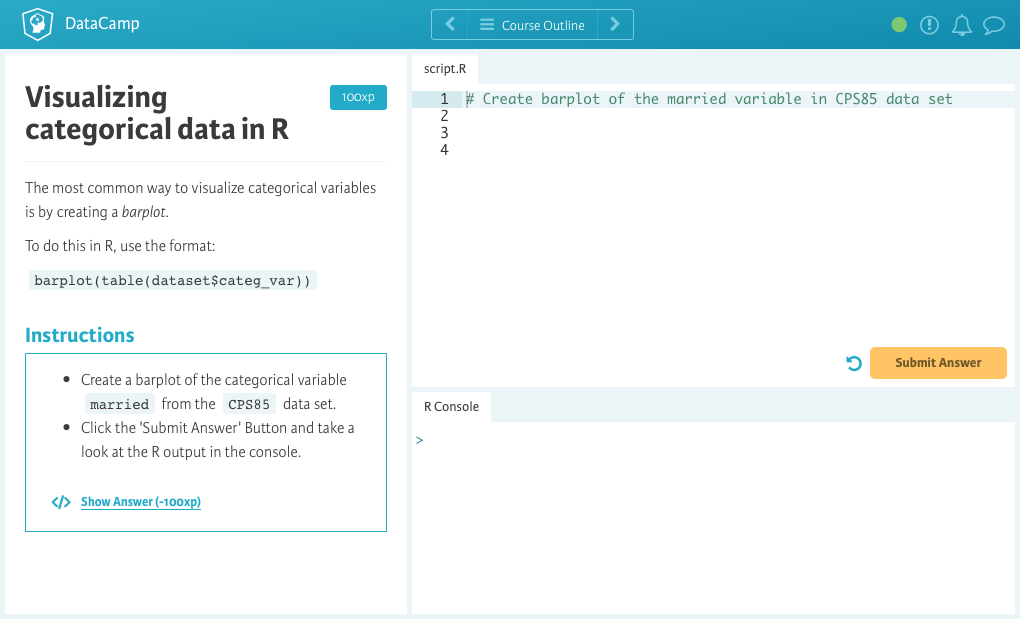
\includegraphics[scale = 0.40] {preview.jpg}
\end{figure}
\subsubsection{Exercise Header}
Whenever a new exercise is added, DataCamp automatically produces the exercise header (---type:, etc.). The header specifies the type
of exercise (\texttt{type}), programming language (\texttt{lang}), available points (\texttt{xp}), skills learned (\texttt{skills}) and a \texttt{key}. 
The types of exercises include normal coding, video, and multiple choice exercises; which will be discussed further in the next section. 
DataCamp assigns 100 points \texttt{xp} by default to normal coding exercises but this value can be modified depending on
difficulty level. After students have completed the exercise, they can check their personal profile to see how many points they earned.
The \texttt{skills} portion of the header refers to DataCamp's
eight different skill sets, defined by numbers 1-8. Skills and their corresponding numbers can be found in the DataCamp
documentation \url{https://www.datacamp.com/teach/documentation#tab_gamification}. 
Lastly, the \texttt{key} acts as a unique
identifier for that exercise, allowing you to modify content without losing any student data. 
In Figure 1, the \texttt{type} is Normal, the language is R, the available points is 100xp and the skills learned is 1 (which 
corresponds to R Programming). 

\subsubsection{Exercise Body}
In the \textit{Assignment} portion of the exercise (not labeled but below the header), instructors can add additional information about the assignment that will help
students understand and complete the instructions, which is displayed in the top left panel of Figure 2. The \textit{instructions} section contains the actual task the student is
asked to execute; instructors can also include a \textit{hint} for extra guidance (bottom left panel Figure 2). The \textit{pre-exercise code} sets up the work space for 
the student - this section contains code to import data sets, install packages and any other operation that you want to be available but not visible to
students. The \textit{sample code} section will contain code or notes that will be visible to students in the R script panel (top right figure 2). Students also use the R script panel to write code that solves the tasks in the instructions. The correct answer to an exercise is coded in the \textit{solution} section
and when a student clicks the \texttt{Submit Code} button, their answer passes through the R console, and then the Submission Correctness Testing (SCT) code where their answer is checked for errors.

\subsubsection{Submission Correctness Test}
The submission correctness testing code (or SCT) automatically assesses if the correct code was submitted. If a student submits an 
incorrect answer, they will receive immediate feedback on what they are doing wrong and the system will guide them to the right answer.
DataCamp provides a helpful R package called \textit{testwhat} which acts as a guide to writing and using SCTs - available on DataCamp's GitHub 
repository: \url{https://github.com/datacamp/testwhat/wiki}. 
The \textit{testwhat} package contains functions that test different types of problems including loops, object definitions, printed output, functions, and other R programming problems.
The submission correctness testing code compares the ideal answer (from the solution code) to the students answer. Various
arguments can be added to the test functions to adjust the testing process and feedback.
Instructors can either use the default feedback that DataCamp automatically generates or write their own custom messages. For example, figure blank
contains the default feedback for a few possible incorrect submissions of the \texttt{hist()} function. 
Suppose the data set is called \texttt{birthdata} and the variable of interest is \texttt{weight}. 


\begin{figure}
\caption{Examples of DataCamps Default Feedback}
\begin{Verbatim}

It's weird but I get errors when I name the data set birth_data.

Student types:                  Default message:


histogram(birthdata$weight)    Have you called hist()?

hist(weight)                    Check your call of hist(). Did you 
                                correctly specify the argument x? 
                                Evaluating the expression you specified
                                caused an error.
   

hist(birthdata$wieght)         Check your call of hist(). Did you
                                correctly specify the argument x? It is
                                a NULL, while it should be a numeric vector.

\end{Verbatim}
\end{figure}

\textit{I might want to add one where student types something with the wrong symbol but I can't get onto the datacamp course for some reason.}

DataCamp's default feedback is meaningful and specific so a lot of the time custom 
messages are not necessary.
However, if students are struggling with a common problem then unique feedback can be very beneficial.

\subsection{DataCamp Exercise Types}
DataCamp courses may contain 3 different types of exercises: Normal coding, video, and multiple choice exercises.
\subsubsection{Normal Exercise}
A \texttt{NormalExercise} is an exercise that prompts a user to submit code. The components of this include: lesson section, instructions, pre-exercise code, sample code, hint, solution and submission correctness testing code (SCT). However, the interface for students (or the \texttt{Preview}
mode) will only include the lesson, instructions, R script panel and R console panel (Figure~\ref{fig:code1}).
\subsubsection{Video Exercise}
Video exercises act as instructional videos that accompany a DataCamp course. Instructors can add short videos of them explaining concepts while 
relevant slides appear in the background. The DataCamp website provides 
more detail on the content of video exercises. 

\subsubsection{Multiple Choice Exercise}

The \texttt{MultipleChoiceExercise}, as you would expect, contains a question and a list of various answers. 
DataCamp offers two types of multiple choice questions: simple and regular. 
The simple multiple choice exercises are used for questions that do not require the R console or any R output. Regular multiple choice exercises 
allow instructors to pre-program objects or plots that the student needs to access to answer the question. Both types of multiple choice exercises 
are straight forward to write can act as quick checks for understanding throughout the chapter.
\begin{figure}
\caption{Example of Multiple Choice - This should be in section 3.4.3}
\begin{Verbatim}[frame=single]
--- type:PlainMultipleChoiceExercise lang:r xp:50 skills:1
    key:9707072219

## Quick check 2

What can R be used for?

*** =instructions
- Graphing data
- Analyzing data
- Calculations
- All of the above
*** =hint
R software can be used for all of these things.
*** =pre_exercise_code
```{r}
```
*** =sct
```{r}
msg_bad <- "That is not correct"
msg_success <- "Exactly! R can do all of these things."
test_mc(correct = 4, 
    feedback_msgs = c(msg_bad, msg_bad, msg_bad, msg_success))
```
\end{Verbatim}
\end{figure}
Similar to \texttt{normal} coding exercises, the lesson, instructions, hint, pre-exercise 
code and SCTs are included in the teach editor. However, multiple choice exercises do not have sample or solution code. 
Instructors write the questions in the lesson
portion of the exercise and offer solutions in the \textit{Instructions} section. Figuremultichoice is an example of plain multiple choice question. ADD PICTURE OF CORRESPONDING PREVIEW FOR MC QUESTION

\begin{verbatim}
Multiple choice exercises use the SCT function called  \texttt{test_mc} 
which requires two arguments: \texttt{correct} and \texttt{feedback_msgs}. 
The \texttt{correct} argument specifies the position of the correct answer;
if the correct answer is the second option listed, then set \texttt{correct = 2}. 
The \texttt{feedback_msgs} argument is a vector of strings that contain feedback 
messages corresponding to the positions of the listed options.

\end{verbatim}
\subsection{Advise for smoother course development}
DataCamp is fairly new and the only available information about course creation is on the DataCamp website. While the documentation on DataCamp is comprehensive, here are some tips for developing a first course.

\subsubsection{GitHub repositories}
When creating your first DataCamp course, it is helpful to view the code from existing community courses. 
The DataCamp repository on GitHub contains links to the course code from several of their available courses. One of the most helpful links for DataCamp beginners
is \url{https://github.com/datacamp/courses-intro-to-r} which contains the source files for the \textit{Introduction to R} course.
You can use these files as a guide to build your own course or even duplicate the file and tailor the content to fit specific needs.

\subsubsection{Collaboration for course development}
To add collaborators to the course, go to the course repository
on GitHub and under \texttt{Settings} you can enter the user names of collaborators. Collaborators who are not the primary author need 
to uncheck `My Courses' in order to view and contribute to the repository.
\subsubsection{Integrating R packages}
Information on how to add data sets and images to a course
can be found in DataCamps \textit{Teach} documentation \url{https://www.datacamp.com/teach/documentation} under the `Upload Assets' tab. However,
there is currently no information on DataCamp about integrating R packages. To use R packages in a course, you will need to create a new file
in the GitHub course repository named \texttt{requirements.r}. This file should contain a line of code with three components: \texttt{devtools::install\_version}, package name and version for 
every package you wish to include in the DataCamp course. For example, the following code will add the \texttt{ggplot2} and \texttt{mosaic} packages to the repository.

\begin{verbatim}
devtools::install_version("ggplot2", "2.2.0")
devtools::install_version("mosaic", "0.14.4")
\end{verbatim}
In order for DataCamp to recognize this new file, you will need to add: \\ \texttt{from: r-base-prod:27} \\ to the \texttt{course.yml} file.

\subsubsection{TeX typesetting or Markdown}
LaTeX is compatible with DataCamp; course builders can use LaTeX math symbols to display Greek letters, formulas, ect. For example:
\begin{verbatim}
$H_0$: $p = 0.07$
$H_a$: $p \neq 0.07$
\end{verbatim}

translates to:

$H_0$: $p = 0.07$

$H_a$: $p \neq 0.07$

\section{Conclusion}

\bibliographystyle{plainnat}
\bibliography{library}




\end{document}
